\documentclass[10pt,a4paper]{article}
% Harava Mobile app user guide. Built with:  pdflatex mobile_guide.tex  (three times, for the contents)
% The screenshots are in guide_img/m_*.jpg (the phone app at 390 x 844 CSS pixels, light theme, Mask addresses on,
% without the map background) and a_workbench.jpg / a_wb_rule.jpg (the full site's Workbench), all taken with the
% author's own Fieldwatch log of 8 November 2026. Same look as the Harava user guide.
\usepackage[T1]{fontenc}
\usepackage[utf8]{inputenc}
\usepackage{mathptmx}
\usepackage[scaled=.92]{helvet}
\usepackage{courier}
\usepackage{microtype}
\usepackage[a4paper,margin=2.0cm,top=2.3cm,bottom=2.2cm,headsep=0.5cm]{geometry}
\usepackage{graphicx}
\usepackage{xcolor}
\usepackage{booktabs}
\usepackage{tabularx}
\usepackage{array}
\usepackage{enumitem}
\usepackage{caption}
\usepackage{float}
\usepackage{fancyhdr}
\usepackage{textcomp}
\usepackage{amsmath}
\usepackage{amssymb}
\usepackage{tikz}
\usepackage{xurl}
% the phone app's symbols, drawn (pdfLaTeX fonts do not have them)
\newcommand{\glyph}[1]{\tikz[baseline=-0.6ex,line width=0.55pt,line cap=round]{#1}}
\DeclareUnicodeCharacter{2630}{\glyph{\foreach \y in {-0.11,0,0.11}{\draw (-0.13,\y)--(0.13,\y);}}}%  ☰ menu
\DeclareUnicodeCharacter{263E}{\glyph{\fill (0,0) circle (0.12); \fill[white] (0.06,0.03) circle (0.1);}}%  ☾ dark
\DeclareUnicodeCharacter{2600}{\glyph{\draw (0,0) circle (0.055); \foreach \a in {0,45,...,315}{\draw (\a:0.09)--(\a:0.14);}}}%  ☀ light
\DeclareUnicodeCharacter{25D0}{\glyph{\draw (0,0) circle (0.12); \fill (0,0.12) arc (90:270:0.12)--cycle;}}%  ◐ auto
\DeclareUnicodeCharacter{2302}{\glyph{\draw (-0.1,-0.11)--(-0.1,0.02)--(0,0.12)--(0.1,0.02)--(0.1,-0.11)--cycle;}}%  ⌂ home
\DeclareUnicodeCharacter{2715}{\ensuremath{\times}}%  ✕
\DeclareUnicodeCharacter{2605}{\ensuremath{\bigstar}}%  ★
\DeclareUnicodeCharacter{2197}{\ensuremath{\nearrow}}%  ↗
\DeclareUnicodeCharacter{22EE}{\ensuremath{\vdots}}%  ⋮
\DeclareUnicodeCharacter{FF0B}{+}%  ＋
\DeclareUnicodeCharacter{2039}{\guilsinglleft}%  ‹
\DeclareUnicodeCharacter{203A}{\guilsinglright}%  ›
\usepackage[hidelinks]{hyperref}

\definecolor{accent}{HTML}{0369A1}
\definecolor{boxbg}{HTML}{F1F6FA}
\definecolor{warnbg}{HTML}{FFF7E8}
\definecolor{warn}{HTML}{B45309}
\captionsetup{font=small,labelfont=bf,labelsep=period,justification=justified,singlelinecheck=false}
\setlist{itemsep=1.5pt,topsep=3pt,parsep=0pt}
\setlength{\parindent}{0pt}
\setlength{\parskip}{4.5pt plus 1pt}
\renewcommand{\arraystretch}{1.15}
\setcounter{tocdepth}{2}
\pagestyle{fancy}
\fancyhf{}
\fancyhead[L]{\small\itshape Harava Mobile app --- what your phone heard, in your pocket}
\fancyhead[R]{\small\itshape Mobile app user guide, version 1.1 --- November 2026}
\fancyfoot[C]{\small\thepage}
\renewcommand{\headrulewidth}{0.3pt}
\hypersetup{pdftitle={Harava Mobile app - User guide},pdfauthor={Otso Laakso, OH2GAX}}

\newcommand{\ui}[1]{\textsf{\small #1}}            % a word on the screen: button, switch, card title
\newcommand{\lead}[1]{\textbf{#1}\enspace}           % run-in paragraph head
\newcommand{\fig}[3]{\begin{figure}[H]\centering\includegraphics[width=#2\textwidth]{guide_img/#1}\caption{#3}\end{figure}}
% three phone screens side by side: \phones{img1}{img2}{img3}{label}{caption}
\newcommand{\phones}[5]{\begin{figure}[H]\centering
  \fbox{\includegraphics[width=0.29\textwidth]{guide_img/#1}}\hfill
  \fbox{\includegraphics[width=0.29\textwidth]{guide_img/#2}}\hfill
  \fbox{\includegraphics[width=0.29\textwidth]{guide_img/#3}}
  \caption{#5}\label{#4}\end{figure}}
% two phone screens: \phonestwo{img1}{img2}{label}{caption}
\newcommand{\phonestwo}[4]{\begin{figure}[H]\centering
  \fbox{\includegraphics[width=0.29\textwidth]{guide_img/#1}}\hspace{1.2cm}
  \fbox{\includegraphics[width=0.29\textwidth]{guide_img/#2}}
  \caption{#4}\label{#3}\end{figure}}
\setlength{\fboxsep}{0pt}\setlength{\fboxrule}{0.4pt}
\newcommand{\infobox}[2]{\par\smallskip\noindent{\setlength{\fboxsep}{3pt}\fcolorbox{accent!60}{boxbg}{\begin{minipage}{\dimexpr\textwidth-6pt-0.8pt\relax}\small
  \textbf{#1}\enspace #2\end{minipage}}}\par\smallskip}
\newcommand{\warnbox}[2]{\par\smallskip\noindent{\setlength{\fboxsep}{3pt}\fcolorbox{warn!60}{warnbg}{\begin{minipage}{\dimexpr\textwidth-6pt-0.8pt\relax}\small
  \textbf{#1}\enspace #2\end{minipage}}}\par\smallskip}

\begin{document}
\thispagestyle{plain}
\begin{center}
{\small Harava project \quad$\cdot$\quad Mobile app user guide, version 1.1 \quad$\cdot$\quad 9 November 2026}\par\vspace{10pt}
{\LARGE\bfseries Harava Mobile app}\par\vspace{5pt}
{\large\bfseries The map, the day, the watch list, every radio, the phone check and uploads ---\\ on your phone, one view at a time}\par\vspace{8pt}
{\normalsize Otso Laakso (OH2GAX)}\par
{\small \texttt{https://harava.oh2gax.org/app} \quad$\cdot$\quad the same style as the WSPR Logger phone app}
\end{center}
\vspace{2pt}

\infobox{In short.}{The Harava Mobile app is Harava made for a phone screen. It is not a separate program to install: it is the page \texttt{/app} of your Harava site, which you can add to the home screen so that it opens like an app. It shows the same data, with the same sign-in and the same permissions, as the full site --- in the style of the WSPR Logger phone app:
\begin{itemize}[leftmargin=1.2em]
\item a slim \textbf{top bar}, \textbf{one view at a time} on the whole screen, and every choice in the \textbf{\ui{☰} menu} (Sections~\ref{sec:screen}--\ref{sec:filter});
\item \textbf{Map}, \textbf{Day} and \textbf{Watch list} --- what was around you, when, and what deserves a closer look (Sections~\ref{sec:map}--\ref{sec:watch});
\item \textbf{Devices} and a page for every radio, with \ui{＋ My device} (Section~\ref{sec:devices});
\item the classroom \textbf{Phone check} and the \textbf{Identification} summary (Sections~\ref{sec:phone}--\ref{sec:ids});
\item \textbf{Imports}: upload Fieldwatch exports straight from the phone that made them (Section~\ref{sec:imp});
\item for admins, the \textbf{Workbench}: the radios Harava cannot name yet, notes, and new rules (Section~\ref{sec:wb}).
\end{itemize}
How to collect with Fieldwatch, and what the data can and cannot tell, is in the \emph{Harava -- User guide}; this guide is about the phone app.}

\infobox{About the figures.}{The screenshots are from the phone app with the author's own Fieldwatch log of 8 November 2026 (a day at home with two short car trips), on a phone screen 390 points wide. They were taken in the light theme (one in the dark theme), with \ui{Mask addresses} on --- the second half of every address and all Wi-Fi names are hidden --- and \emph{without the map background}: the map shows only the path and the pins on a plain surface. On your phone the map has streets under them. The numbers on your phone will be different.}

\tableofcontents
\bigskip

% ─────────────────────────────────────────────────────────────────────
\section{Opening the app}\label{sec:open}

\lead{The address.} Open your Harava site with \texttt{/app} at the end, for example \url{https://harava.oh2gax.org/app}. Sign in with your own username and password, the same as on the full site (\ui{Keep me signed in} remembers you on the phone for 30 days). Without a sign-in the app goes to the sign-in page and comes back after it.

\lead{Add it to the home screen.} Then it opens with one tap, on the whole screen, without the browser's address bar:
\begin{itemize}[leftmargin=1.2em]
\item \textbf{Android, Chrome:} \ui{⋮} (top right) $\rightarrow$ \ui{Add to Home screen} (or \ui{Install app}) $\rightarrow$ \ui{Add}.
\item \textbf{iPhone, Safari:} the Share button $\rightarrow$ \ui{Add to Home Screen} $\rightarrow$ \ui{Add}.
\end{itemize}
The icon is Harava's rake. The app remembers the view you used last, the day and all the options, on that phone.

\lead{Your permission.} What you can do depends on the permission the admin gave you (Table~\ref{tab:perm}). Buttons you cannot use are not shown.

\begin{table}[H]\small\centering
\caption{The three permissions in the phone app.}\label{tab:perm}
\begin{tabularx}{\textwidth}{>{\bfseries}p{2.2cm}X}
\toprule
Permission & In the phone app you can \dots\\
\midrule
View only & look at every view: Map, Day, Watch list, Devices, every radio's page, Phone check, Identification and the list of imports.\\
Analyze & also upload Fieldwatch exports, switch imports on or off, delete them, and mark radios as \emph{My devices}.\\
Admin & also use the Workbench (Section~\ref{sec:wb}), and open the full site's Workbench and Maintenance pages from the menu.\\
\bottomrule
\end{tabularx}
\end{table}

\lead{The full site.} \ui{Full site ↗} at the bottom of the menu opens the normal Harava page. Some things are done there only: the CSV export, editing the list of My devices, time windows within a day, and user management (admins).

% ─────────────────────────────────────────────────────────────────────
\section{The screen}\label{sec:screen}

\phones{m_map.jpg}{m_menu.jpg}{m_menu_general.jpg}{fig:screen}{The Map view with the status card at the bottom (left); the \ui{☰} menu with the day, the views as tiles and the Filter section (middle); the General section at the bottom of the menu (right).}

\lead{The top bar} (Figure~\ref{fig:screen}, left) has, from the left:
\begin{itemize}[leftmargin=1.2em]
\item \ui{☰} --- opens the menu. A red dot on it means that \emph{What's new} has something you have not read.
\item the \textbf{name of the view} and, under it, the \textbf{day} it shows (\emph{all days} for Imports and the Workbench);
\item the \textbf{time} on your phone (\emph{local});
\item the \textbf{theme} button: a tap steps \emph{Dark} (☾) $\rightarrow$ \emph{Light} (☀) $\rightarrow$ \emph{Auto} (◐, follows the phone's own setting). It is the same setting as on the full site.
\item a \textbf{dot} for how new the data is: \emph{green} when the newest hear is less than 6 hours old, \emph{amber} within 2 days, \emph{red} older. Its age is also written in the General section.
\end{itemize}

\lead{One view at a time.} The view fills the screen below the bar. Scroll it with your finger; the map is moved and zoomed with your fingers as usual.

\lead{The Back button} of the phone closes the menu or an open window first, and otherwise goes to the view you came from --- for example from a radio's page back to the Devices list.

\lead{Short messages} (\emph{Saved}, \emph{Could not load: \dots}) appear for a few seconds at the bottom.

\lead{New versions.} When Harava on the server is updated, or when the app comes back after more than an hour in the background, it loads itself again. You never have to clear anything; the view and the options stay.

% ─────────────────────────────────────────────────────────────────────
\section{The menu}\label{sec:menu}

The \ui{☰} menu (Figure~\ref{fig:screen}, middle) slides in from the left. From the top:
\begin{enumerate}[leftmargin=1.4em]
\item \textbf{Day} --- \ui{‹} and \ui{›} step one day back or forward; the list in the middle has every day with data, with its number of hears, and \emph{All days}. \ui{Until} makes it a range of several days (the steps then move the whole range). The day applies to every view except Imports and the Workbench.
\item \textbf{Whose data} --- shown when there is more than your own: \emph{My data + shared with me} (the default), \emph{My data only}, one user's shared data, or for admins \emph{All users}. It is the same choice as on the full site.
\item \textbf{The views} as tiles: Map, Day, Watch list, Devices, Phone check, Identification, Imports and, for admins, Workbench. The view on the screen is highlighted. A tap changes the view and closes the menu.
\item \textbf{Options}, one folding section per view. The section of the view on the screen opens by itself and the others stay folded; tap a title to open or fold it. The \emph{Filter} section belongs to Map, Day, Watch list and Devices.
\item \textbf{General} (Figure~\ref{fig:screen}, right): who is signed in and with which permission, the \ui{Mask addresses} switch (Section~\ref{sec:mask}), a short help, the newest data, and the buttons \ui{What's new}, \ui{About}, \ui{User guides}, \ui{My account} (change your password), \ui{Sign out}, and for admins \ui{Workbench (full site)} and \ui{Maintenance}. \ui{Full site ↗} opens the normal page.
\end{enumerate}
A choice made with a row of \emph{chips} (round buttons) or a \emph{switch} takes effect at once and is remembered on the phone. Close the menu with \ui{✕}, by tapping the dimmed view beside it, or with Back.

% ─────────────────────────────────────────────────────────────────────
\section{The filter}\label{sec:filter}

\begin{figure}[H]\centering
\begin{minipage}[c]{0.30\textwidth}\centering\fbox{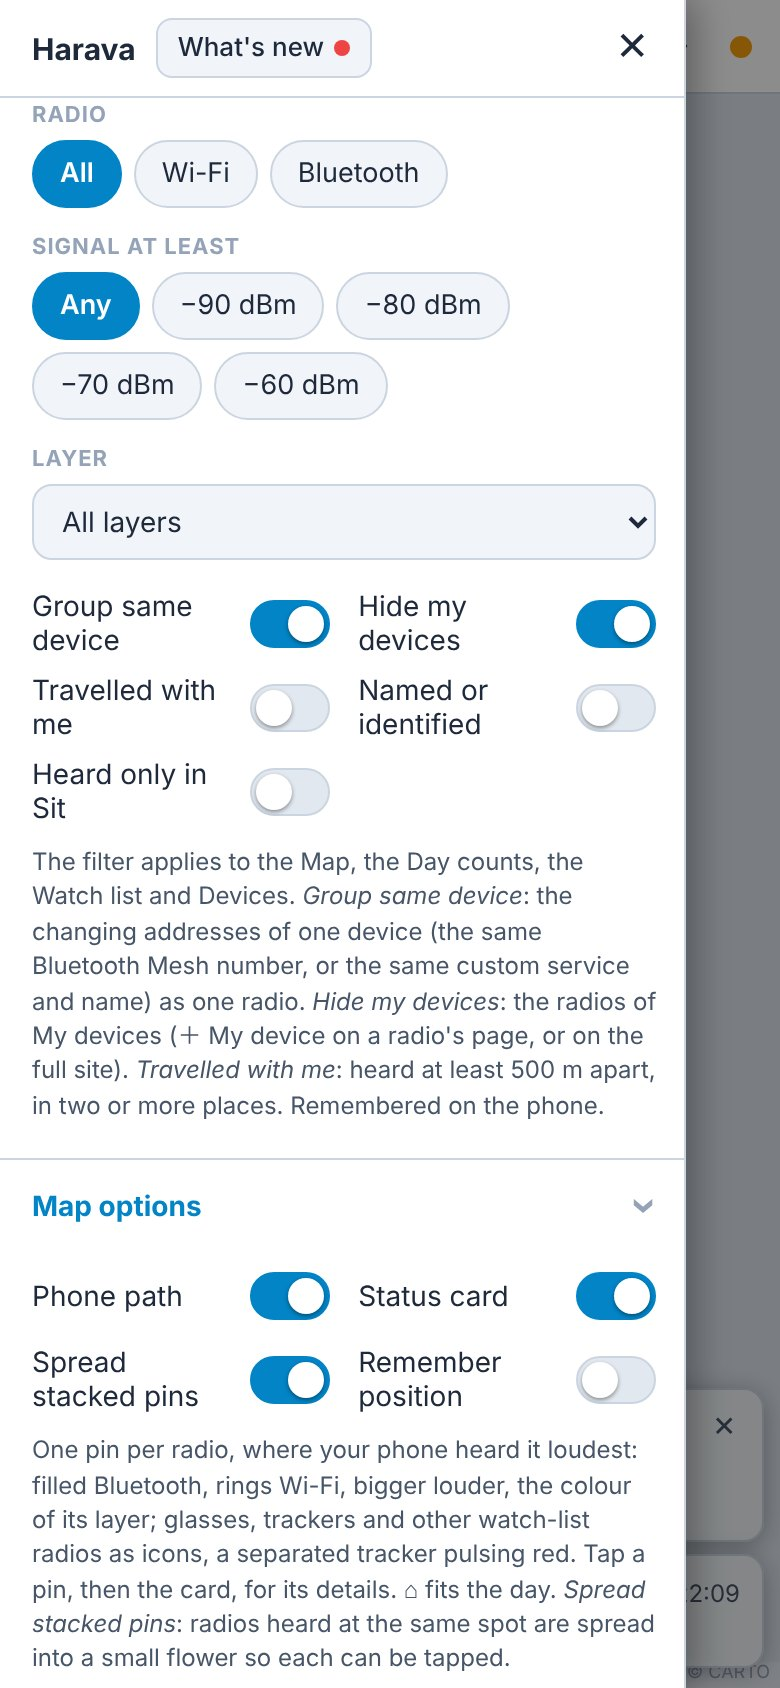
\includegraphics[width=\textwidth]{guide_img/m_menu_filter.jpg}}\end{minipage}\hfill
\begin{minipage}[c]{0.64\textwidth}\small
\textbf{Radio} --- \ui{All}, \ui{Wi-Fi} or \ui{Bluetooth}.\par\smallskip
\textbf{Signal at least} --- only radios heard at least this strong at some moment: \ui{Any}, $-90$ to $-60$\,dBm. $-60$\,dBm or more is usually within a few metres.\par\smallskip
\textbf{Layer} --- one device layer only, for example \emph{Tracker} or \emph{Home \& IoT}; the numbers tell how many the other choices leave.\par\smallskip
\textbf{Group same device} --- the changing Bluetooth addresses of one device as one radio, when Harava has proof that they belong together. On by default.\par\smallskip
\textbf{Hide my devices} --- leaves out your own devices (\emph{My devices}). On by default.\par\smallskip
\textbf{Travelled with me} --- only radios heard in two or more places at least 500\,m apart: devices in your car or bag, or someone travelling with you.\par\smallskip
\textbf{Named or identified} --- only radios that tell a name, have a Fieldwatch signature or are identified by Harava.\par\smallskip
\textbf{Heard only in Sit} --- only radios that only a Sit export has (the log missed them).
\end{minipage}
\caption{The Filter section and the Map options in the menu.}\label{fig:filter}
\end{figure}

The filter applies to the Map, the Day counts, the Watch list (except the layer choice) and Devices. The full site's sidebar has the same filter; the two are set separately.

% ─────────────────────────────────────────────────────────────────────
\section{Map}\label{sec:map}

\phonestwo{m_map.jpg}{m_sel.jpg}{fig:map}{The Map: your path (dashed blue) and one pin per radio; the status card at the bottom (left). A tapped pin gets an amber ring and a card with its name, signal and layer (right); a tap on the card opens the radio's own page.}

\lead{What is on it.} The dashed blue line is your phone's path on the chosen day. Every radio has \emph{one pin}, at the place where your phone heard it loudest: filled dots are Bluetooth, rings are Wi-Fi, a bigger pin was louder, and the colour is its layer. Watch-list radios --- glasses, trackers, surveillance, police, drones and hacking tools --- are icons, and a tracker separated from its owner pulses red. A pin is where \emph{your phone} was, not where the radio is.

\lead{Tap a pin} (Figure~\ref{fig:map}, right): a card shows its name (or address), strongest signal, kind, layer and identification. \ui{Details ›} (a tap anywhere on the card) opens the radio's page (Section~\ref{sec:devices}); \ui{✕} or a tap on the empty map closes the card.

\lead{⌂} under the zoom buttons fits the whole day on the screen.

\lead{The status card} at the bottom tells the day, the time of the newest data, how many radios the filter leaves (Wi-Fi and Bluetooth separately) and how many are on the watch list.

\lead{Map options} (in the menu, Figure~\ref{fig:filter}):
\begin{itemize}[leftmargin=1.2em]
\item \ui{Phone path} --- show or hide the path;
\item \ui{Status card} --- show or hide the card at the bottom;
\item \ui{Spread stacked pins} --- radios heard at the very same spot (all of a home's radios, for example) are spread into a small flower, so each can be tapped;
\item \ui{Remember position} --- the map opens where you left it, instead of fitting the day.
\end{itemize}

% ─────────────────────────────────────────────────────────────────────
\section{Day}\label{sec:day}

\phones{m_day.jpg}{m_day2.jpg}{m_dark.jpg}{fig:day}{The Day view: the counts and the hears per 10 minutes (left); the device layers and the most common identifications (middle); the same in the dark theme (right).}

The Day view tells the whole day in numbers (Figure~\ref{fig:day}):
\begin{itemize}[leftmargin=1.2em]
\item \textbf{the counts} --- radios, hears, the hours with data, Wi-Fi and Bluetooth, how many Bluetooth radios are \emph{identified} (by Fieldwatch or Harava), trackers (and how many of them were separated from their owner), glasses \& VR, and radios that travelled with you;
\item \textbf{Hears per 10 min} --- the bars are hears (Wi-Fi blue, Bluetooth green) and the line is radios heard for the first time that day. A spike of new radios is a new place or a crowd. In the menu, \ui{Day options} $\rightarrow$ \ui{Timeline shows} limits the graph to one layer, for example \emph{Glasses \& VR}: then you see exactly when such a radio was near;
\item \textbf{Device layers} --- how many radios of each layer; \emph{tap a layer} to list its radios in Devices;
\item \textbf{Identified as} --- the ten most common identifications; \emph{tap one} to list those radios in Devices.
\end{itemize}

% ─────────────────────────────────────────────────────────────────────
\section{Watch list}\label{sec:watch}

\begin{figure}[H]\centering
\begin{minipage}[c]{0.30\textwidth}\centering\fbox{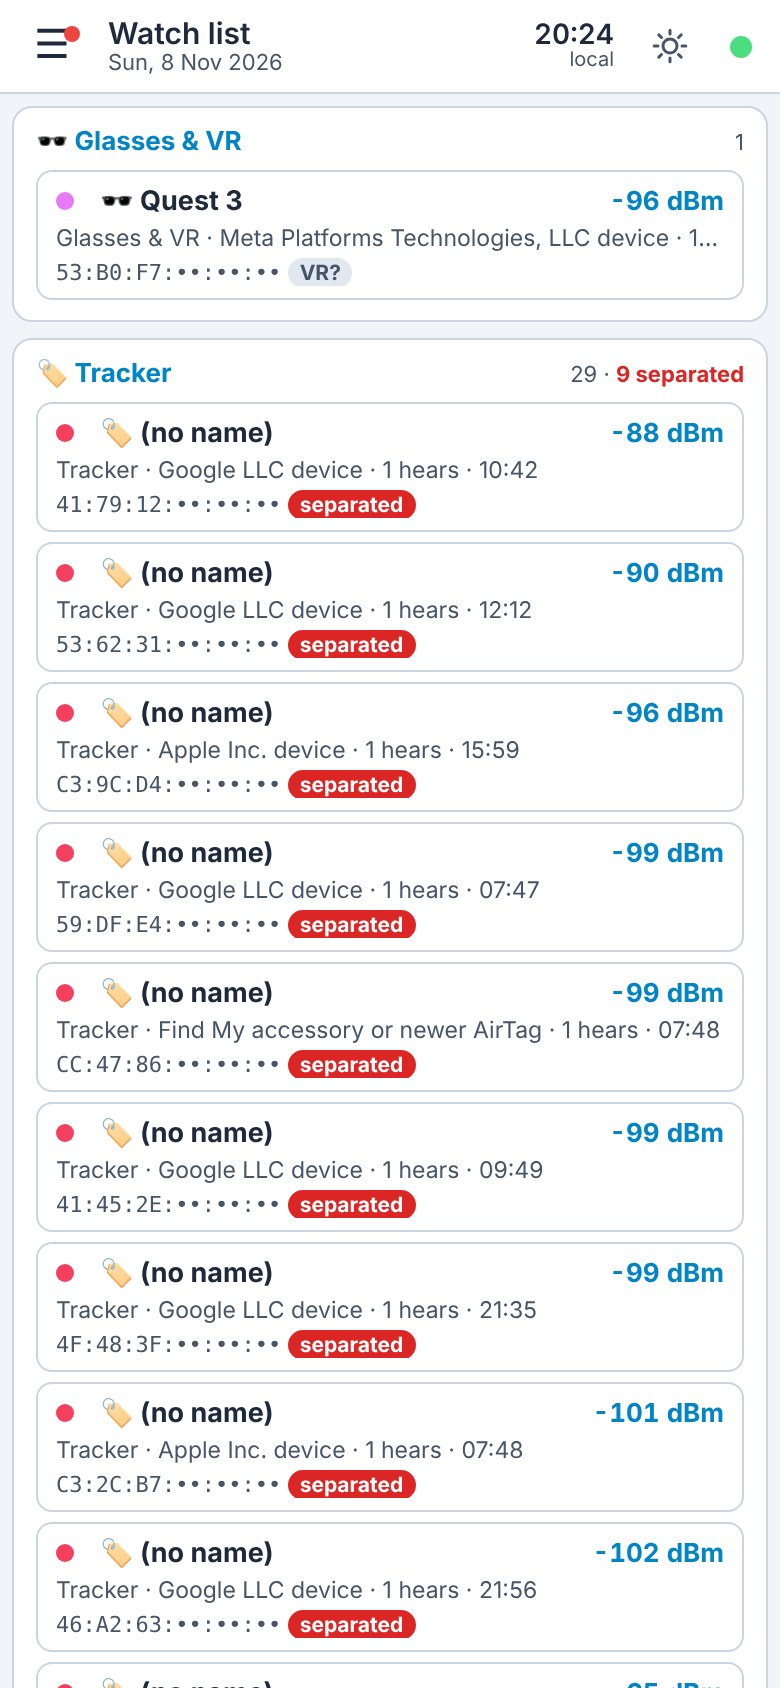
\includegraphics[width=\textwidth]{guide_img/m_watch.jpg}}\end{minipage}\hfill
\begin{minipage}[c]{0.64\textwidth}\small
The Watch list collects the radios that deserve a closer look, layer by layer: \textbf{Glasses \& VR}, \textbf{Tracker}, \textbf{Surveillance}, \textbf{Police / body cam}, \textbf{Drone} and \textbf{Hacking tool}. The heading of each tells how many were heard, and how many trackers were \emph{separated}.\par\smallskip
In each layer the separated trackers come first, then the strongest. A row shows the name, the strongest signal, the layer, the identification, the number of hears, the last time, the address and the tags.\par\smallskip
\textbf{Reading it.} A tracker that is \emph{separated} from its owner and heard in several places along your way deserves a closer look --- open it and look at its map. One \emph{near its owner} is normal: someone walked by with their keys. Smart glasses usually advertise without a name; a name such as \emph{Quest~3} adds a \textbf{VR?} tag, since Meta uses one Bluetooth ID for both.\par\smallskip
Tap a row for the radio's page.
\end{minipage}
\caption{The Watch list.}\label{fig:watch}
\end{figure}

% ─────────────────────────────────────────────────────────────────────
\section{Devices and a radio's page}\label{sec:devices}

\phones{m_dev.jpg}{m_device.jpg}{m_device2.jpg}{fig:dev}{Devices: every radio with search (left). A radio's page: what it is (middle), and its signal over time and every place it was heard (right).}

\lead{Devices} (Figure~\ref{fig:dev}, left) lists every radio the filter leaves, 150 at a time (\ui{Show more} at the end). The box at the top searches the name, address, maker, signature, layer, \emph{Identified as} and company --- for example \texttt{hue}, \texttt{tracker} or the start of an address. \ui{Devices options} $\rightarrow$ \ui{Sort by}: \ui{Strongest}, \ui{Most hears}, \ui{Latest}, \ui{Name} or \ui{Layer}.

\lead{Tags} on a row: \textbf{★} one of My devices; \textbf{N addr.} one device with many addresses; \textbf{separated} tracker; \textbf{travelled}; \textbf{VR?}; \textbf{sit only}; a temperature for Ruuvi sensors.

\lead{A radio's page} (Figure~\ref{fig:dev}, middle and right) opens with a tap on a row, a card or a Watch list row. It shows the name and address, its layer and kind, how it was identified (\emph{Identified as}, company, Fieldwatch signatures, maker), how many addresses belong to the same device, the hears, first and last time, strongest and median signal, the places and how far apart they were, the raw advertisement and the days it was heard. Below them:
\begin{itemize}[leftmargin=1.2em]
\item \ui{Show on map} --- back to the map, zoomed to the radio, with its card open;
\item \ui{＋ My device} (Analyze permission) --- marks the radio as yours, with a label you type. A Bluetooth radio with a name is matched by its name (its address changes); others by their address. From then on \ui{Hide my devices} leaves it out, and the Phone check never counts it;
\item \textbf{Signal} --- the signal strength of every hear over the day;
\item \textbf{the map} --- every place your phone heard it (bigger = louder), joined in time order. A radio that follows your path travelled with you; one that stays in one spot was fixed there.
\end{itemize}
Back returns to the list where you were.

% ─────────────────────────────────────────────────────────────────────
\section{Phone check}\label{sec:phone}

\begin{figure}[H]\centering
\begin{minipage}[c]{0.30\textwidth}\centering\fbox{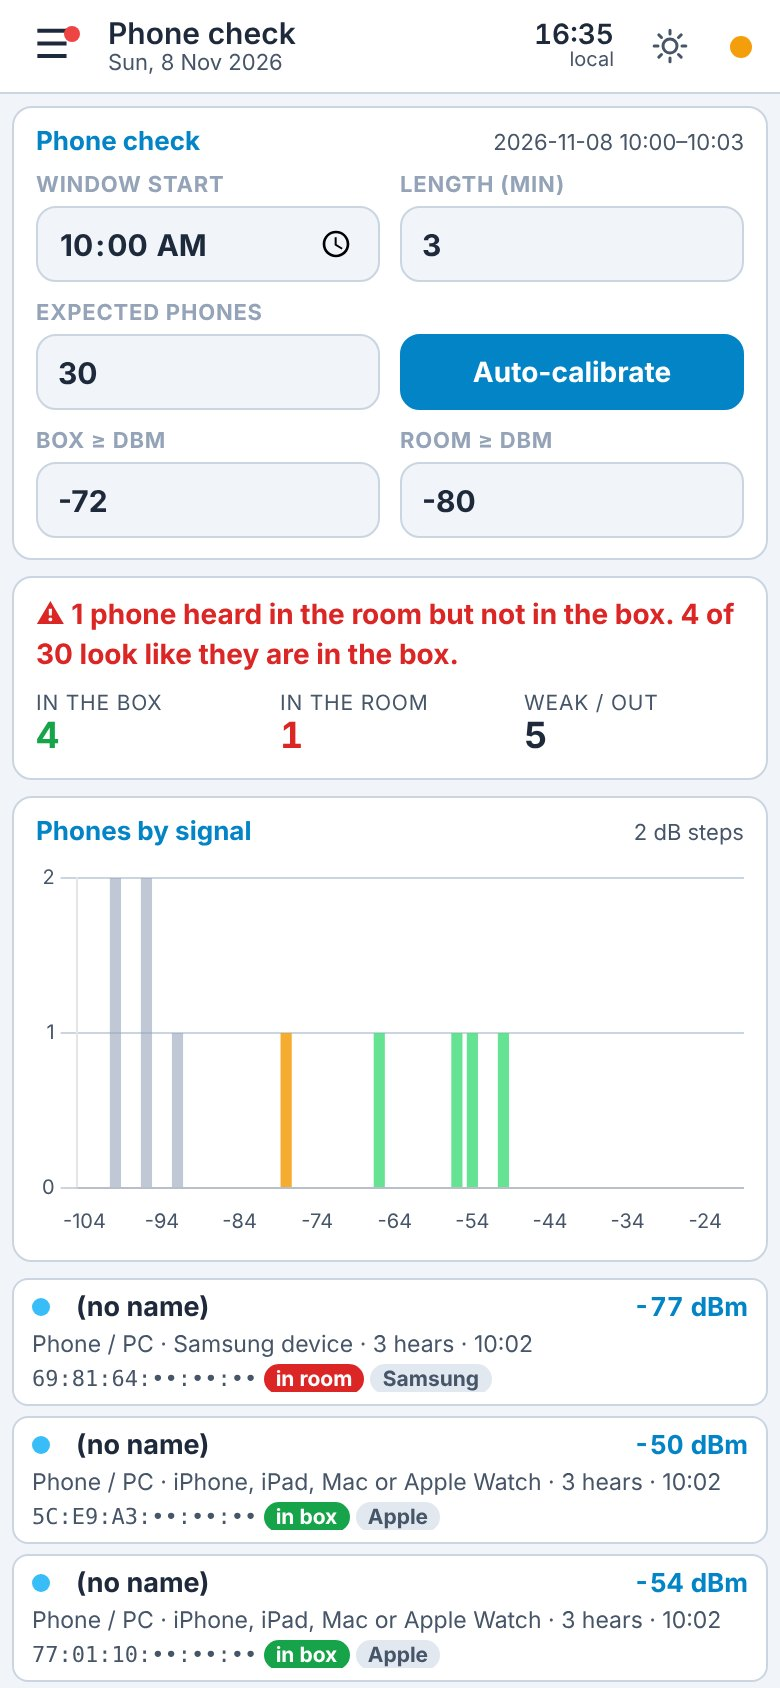
\includegraphics[width=\textwidth]{guide_img/m_phone.jpg}}\end{minipage}\hfill
\begin{minipage}[c]{0.64\textwidth}\small
\textbf{The idea.} At the start of a lesson the students' phones go into a box next to the teacher's phone, which runs Fieldwatch. The check tells whether all phones are in the box, or whether some are still heard elsewhere in the room.\par\smallskip
\textbf{Step by step.}
\begin{enumerate}[leftmargin=1.3em]
\item Import the teacher phone's log (Section~\ref{sec:imp}) and choose its day in the menu.
\item \ui{Window start}: a moment when the phones are in the box; \ui{Length}: 2--5 minutes.
\item \ui{Expected phones}: how many should be in the box.
\item \ui{Auto-calibrate} sets \ui{Box $\geq$ dBm} from the data (just below the expected number of strongest phones, or in a clear gap); \ui{Room $\geq$ dBm} is the weakest signal still counted in the room.
\end{enumerate}
\textbf{The answer.} Green: all phones in the box and nothing else in the room. Red: phones heard in the room but not in the box. Amber: fewer in the box, none elsewhere --- the rest may be off, in flight mode or shielded. Below are the numbers per zone, the phones by signal (green in the box, amber in the room, grey weak) and the list with an \textbf{in box} / \textbf{in room} tag.
\end{minipage}
\caption{The Phone check: a 3-minute window at 10:00 after \ui{Auto-calibrate}.}\label{fig:phone}
\end{figure}

\lead{Phone check options} (in the menu): \ui{Signal of a phone} --- \ui{Strongest} or \ui{Median} hear in the window; \ui{Count Windows PCs}; \ui{Count unknown random} (Bluetooth radios with a random address and no identification). Phones of My devices never count. The check uses the log only, not Sit exports. A metal box blocks the signal: use cardboard or plastic.

% ─────────────────────────────────────────────────────────────────────
\section{Identification}\label{sec:ids}

\begin{figure}[H]\centering
\begin{minipage}[c]{0.30\textwidth}\centering\fbox{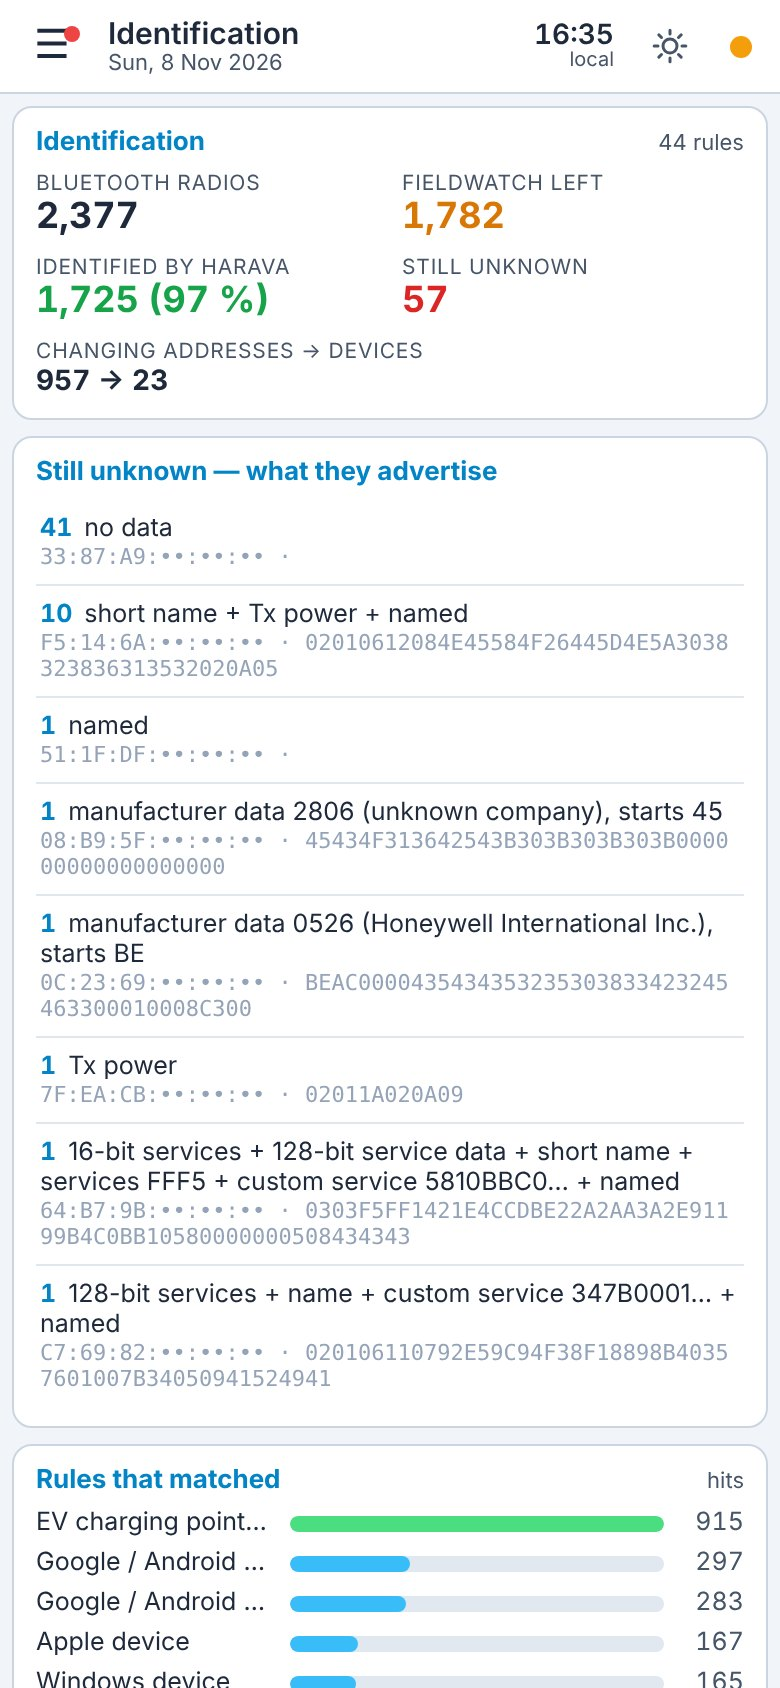
\includegraphics[width=\textwidth]{guide_img/m_ids.jpg}}\end{minipage}\hfill
\begin{minipage}[c]{0.64\textwidth}\small
Harava has its own identification database on top of Fieldwatch's signatures: the official Bluetooth SIG numbers and Harava's own rules. This view tells, for the chosen day:\par\smallskip
\textbf{Identification} --- the Bluetooth radios, how many Fieldwatch left without a signature, how many of those Harava identified, how many are still unknown, and how many changing addresses were joined into how many devices. The number at the top right is the number of rules.\par\smallskip
\textbf{Still unknown --- what they advertise} --- the most common kinds of advertisement among the unknown radios, with an example. These are the next rules to write; admins do it in the Workbench (Section~\ref{sec:wb}).\par\smallskip
\textbf{Rules that matched} --- every rule that named something that day, with the number of radios.
\end{minipage}
\caption{The Identification view.}\label{fig:ids}
\end{figure}

% ─────────────────────────────────────────────────────────────────────
\section{Imports: upload from the phone}\label{sec:imp}

\begin{figure}[H]\centering
\begin{minipage}[c]{0.30\textwidth}\centering\fbox{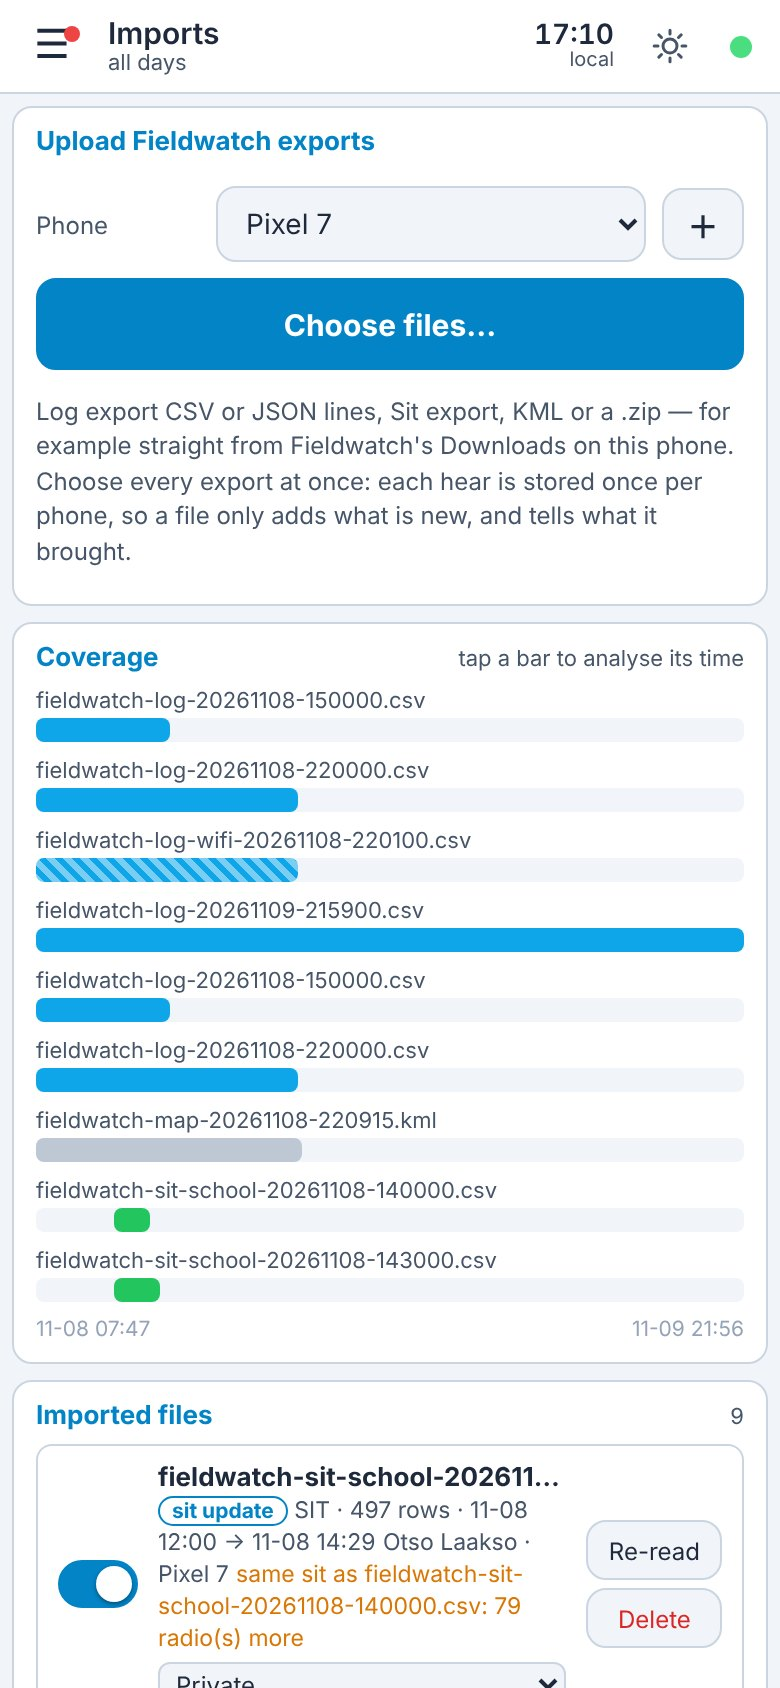
\includegraphics[width=\textwidth]{guide_img/m_imp.jpg}}\end{minipage}\hfill
\begin{minipage}[c]{0.64\textwidth}\small
The phone that ran Fieldwatch can send its exports to Harava straight away (Analyze permission):
\begin{enumerate}[leftmargin=1.3em]
\item In Fieldwatch, export the log (CSV, JSON lines or KML) and, if you sat somewhere, the Sit. Fieldwatch saves them in \emph{Downloads}.
\item In Harava, open \ui{Imports}, check the \ui{Phone} (\ui{＋} adds one) and tap \ui{Choose files…}. Pick one or more files, or a \texttt{.zip} (a long press selects several). Older files are imported first.
\item Harava tells, file by file, what it brought: \textbf{new}, \textbf{extends} (a newer export of the rolling log: most rows were already stored, ``+N'' new), \textbf{overlaps}, \textbf{duplicate} (nothing new) or \textbf{sit update} (a newer export of the same Sit) --- or why a file was skipped or refused.
\end{enumerate}
You can choose every export you have at once: Fieldwatch's log export always contains everything still on the phone, and Harava keeps every hear only once per phone.\par\smallskip
\textbf{Coverage} draws every import as a bar over time (blue log, green Sit, violet KML, grey switched off); tap one to analyse its days.\par\smallskip
\textbf{Imported files}: the switch takes a file in or out of the analysis; \ui{Re-read} reads the kept original again; \ui{Delete} removes it (rows another file also has stay). Under each of your own files, \emph{Private} / \emph{Shared with all users} chooses who else sees it (chosen users on the full site).
\end{minipage}
\caption{Imports: the phone, the upload, and the coverage of every import.}\label{fig:imp}
\end{figure}

% ─────────────────────────────────────────────────────────────────────
\section{Workbench (admins)}\label{sec:wb}

The Workbench is where unknown radios become rules. It is for admins only, and it works on \emph{all days} at once.

\phones{m_wb.jpg}{m_wbd.jpg}{m_wbd2.jpg}{fig:wb}{The Workbench: the kinds of unknown radios (left); one kind with its status and note and its advertisement decoded (middle); its hints, what was heard together with it, and its radios (right).}

\lead{One row is one kind of device.} Every Bluetooth radio Harava cannot name is put in a bucket by \emph{what it advertises}, leaving out its address and the bytes that change: the company and the first byte of its manufacturer data, its service data, a vendor's own 128-bit service, other services and data types --- and the shape of its name only when nothing else tells (\texttt{NEXO\&D]NZ08286152} and \texttt{NEXO\&D]NZ082861VD} both become \texttt{NEXO\&D]\#}). The line above the list tells how many radios of all days are unknown, weakly identified and without data, how much of the newest day is named, and how many kinds have notes.

\lead{Workbench options} (in the menu): \ui{Show} chooses the tab --- \ui{Unknown} (advertising data but no rule), \ui{Weakly identified} (only the company, only a custom service, or a rule marked as a guess) or \ui{No data} (flags only: the rest is in a scan response, which Fieldwatch does not log) --- and \ui{Status} shows only the kinds with that status. The search box finds a pattern, a name or a note.

\lead{A kind's page} (Figure~\ref{fig:wb}, middle and right):
\begin{itemize}[leftmargin=1.2em]
\item how many radios, devices and hears, the strongest signal, the days and the names;
\item \textbf{Status and note} --- \ui{New}, \ui{Investigating}, \ui{Identified}, \ui{Ignore} or \ui{Can't identify}, and a free note: what you know or suspect. \ui{Save} keeps them on the server, for every admin;
\item \textbf{The advertisement, decoded} --- each part of the raw data with its meaning;
\item \textbf{Variants} --- the different raw advertisements, and the \emph{bytes that change} between radios (counters and rotating numbers, which are not part of the pattern);
\item \textbf{Hints} --- what the Bluetooth SIG lists say about the company and the services, whether the radios travelled with you or stayed at one place for days, whether many addresses were few devices; and buttons to search the web, GitHub code (for a vendor's own service number) or the SIG lists;
\item \textbf{Heard together with} --- other radios heard in the same 5-minute slots: a phone app's service next to a gadget may tell whose app it is;
\item \textbf{Radios} --- every address with its signal, hears and days.
\end{itemize}

\begin{figure}[H]\centering
\begin{minipage}[c]{0.30\textwidth}\centering\fbox{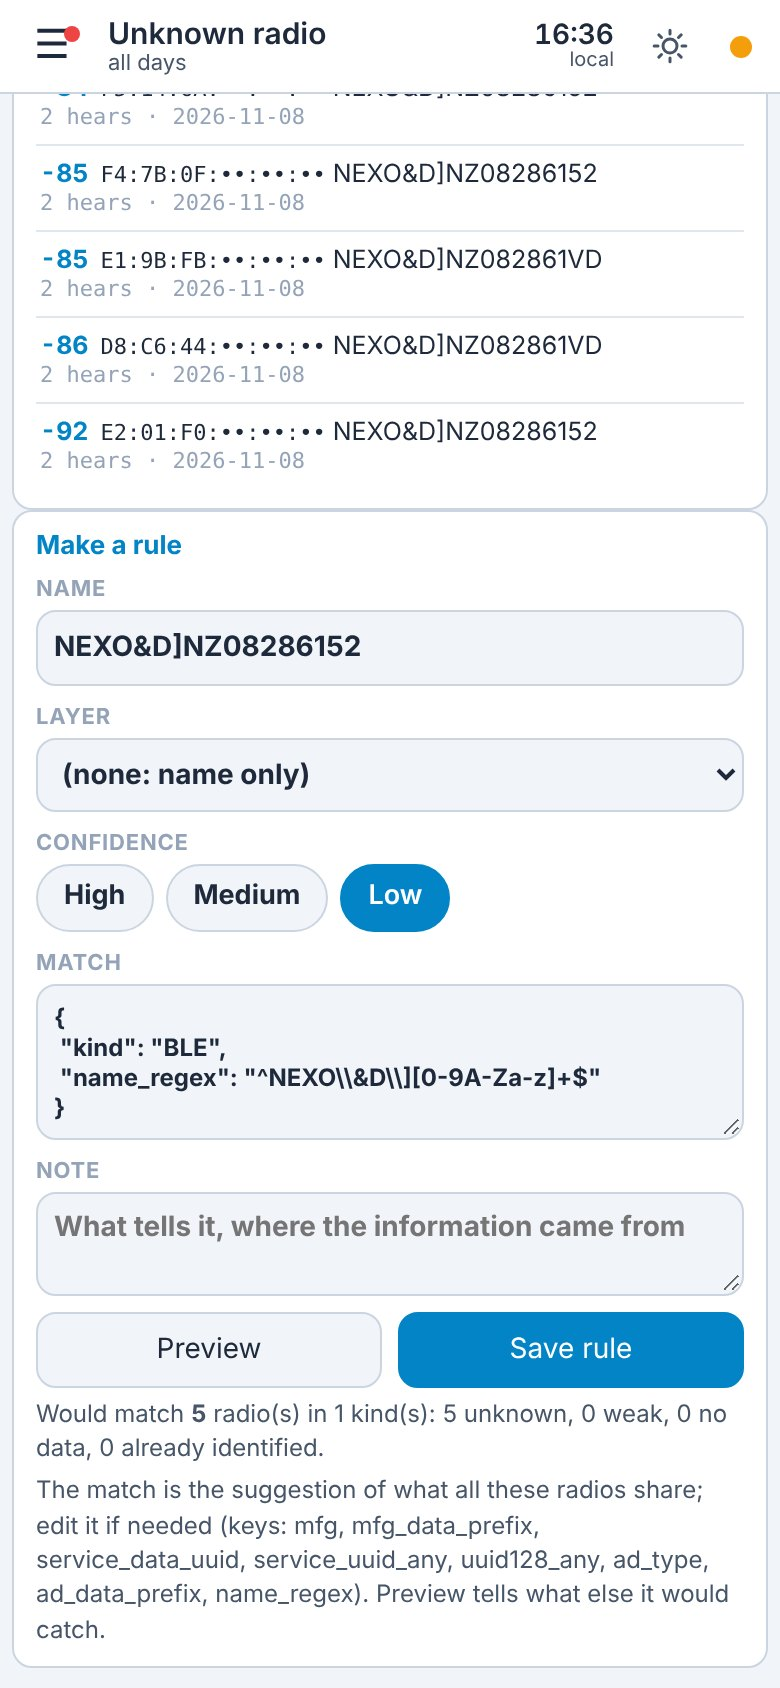
\includegraphics[width=\textwidth]{guide_img/m_wbd_rule.jpg}}\end{minipage}\hfill
\begin{minipage}[c]{0.64\textwidth}\small
\textbf{Make a rule.} When you know what the radios are:
\begin{enumerate}[leftmargin=1.3em]
\item Write the \ui{Name} --- what Harava will show as \emph{Identified as}.
\item Choose a \ui{Layer}, or none to give only the name.
\item Choose the \ui{Confidence}: \emph{High} when the protocol says so, \emph{Medium} when it is typical and well known, \emph{Low} for a likely guess (shown with a ``?'', and still listed under \emph{Weakly identified}).
\item \ui{Match} is filled with what all these radios share. Edit it if needed; the keys are \texttt{mfg}, \texttt{mfg\_data\_prefix}, \texttt{service\_data\_uuid}, \texttt{service\_uuid\_any}, \texttt{uuid128\_any}, \texttt{ad\_type}, \texttt{ad\_data\_prefix} and \texttt{name\_regex}, and all given must hold.
\item \ui{Preview} counts what the rule would catch, of all days --- and warns if it would take over radios that are already identified.
\item \ui{Save rule}. Harava uses it at once, and marks the kind \emph{Identified}.
\end{enumerate}
\end{minipage}
\caption{Making a rule, with the preview of what it would catch.}\label{fig:rule}
\end{figure}

\infobox{Where the rules go.}{Rules made in the Workbench are kept on that server only, in \texttt{ids/local\_rules.json} --- not in git, and copied with the database before every update. They are tried \emph{before} Harava's shared database, so a new rule wins while you try it out. The full site's Workbench (\ui{Workbench (full site)} in the menu, Figure~\ref{fig:wbfull}) lists them, removes them, and has \ui{Export rules and notes}, which downloads the rules and notes as one file: good rules can then be added to the shared database in a later version of Harava.}

\fig{a_workbench.jpg}{0.98}{The full site's Workbench on a computer: the tabs, the kinds and a kind's page side by side, and the progress per day at the top.}\label{fig:wbfull}

% ─────────────────────────────────────────────────────────────────────
\section{What's new, guides, About and masking}\label{sec:mask}

\phonestwo{m_news.jpg}{m_guides.jpg}{fig:sheet}{What's new (left) and User guides (right). The buttons at the top switch between What's new, User guides and About.}

\lead{What's new} (in the menu, or the red-dotted \ui{What's new} beside the name) opens short notes for users, newest version first; older versions are folded. The red dot goes away once you have opened it. \ui{User guides} lists the guides as PDF --- this guide, the Harava User guide and the Admin and server guide --- with \ui{Open PDF} and \ui{Download}. \ui{About} tells what Harava is, who made it and where its source code is.

\lead{Mask addresses} (General section) is for screenshots you share: the second half of every address (\texttt{5C:E9:A3:••:••:••}), all Wi-Fi network names (\emph{Wi-Fi network 1, 2, \dots}) and other people's device names are hidden on the screen. Wi-Fi names with their addresses can be looked up in public Wi-Fi maps, so they could point to a home. The data is not changed; switch it off to see everything again. The setting is the same as on the full site, on that phone.

% ─────────────────────────────────────────────────────────────────────
\section{Troubleshooting}\label{sec:trouble}
\begin{table}[H]\small\centering
\caption{Common situations.}
\begin{tabularx}{\textwidth}{>{\raggedright}p{4.6cm}X}
\toprule
\textbf{What you see} & \textbf{Why, and what to do}\\
\midrule
The sign-in page instead of the app & You were signed out (\ui{Sign out}, a new password, or 30 days passed). Sign in; the app opens again.\\
\emph{Could not load: \dots} & The phone has no connection, or the server is restarting after an update. Try again in a moment.\\
The map has pins but no streets & The map background comes from CARTO over the internet; on a weak connection it comes slowly.\\
The dot at the top is red & The newest data is more than two days old. Upload a new export (Section~\ref{sec:imp}).\\
A view is empty or the counts look small & Check the day and the Filter in the menu --- \ui{Named or identified} or a \ui{Layer} may be on.\\
No \ui{Choose files…} or \ui{＋ My device} & Your permission is \emph{View only}; ask the admin.\\
No Workbench tile & The Workbench is for admins only.\\
\emph{already imported as \dots} & The very same file was imported before; nothing is done twice.\\
The app looks different after an update & It loaded the new version by itself. \ui{What's new} tells what changed.\\
\bottomrule
\end{tabularx}
\end{table}

% ─────────────────────────────────────────────────────────────────────
\section{Quick reference}\label{sec:quick}
\begin{table}[H]\small\centering
\begin{tabularx}{\textwidth}{>{\raggedright}p{5.2cm}X}
\toprule
\textbf{I want to \dots} & \textbf{Do this}\\
\midrule
open the app & \texttt{https://harava.oh2gax.org/app}, or the Harava icon on the home screen\\
change the day & \ui{☰} $\rightarrow$ \ui{‹} \ui{›} or the day list\\
change the view & \ui{☰} $\rightarrow$ a tile\\
see only Bluetooth / strong / one layer & \ui{☰} $\rightarrow$ Filter\\
see what a pin is & tap it, then tap the card\\
find a radio & Devices, the search box\\
see where a radio was heard & its page, the map at the bottom\\
hide my own devices & a radio's page $\rightarrow$ \ui{＋ My device}; Filter $\rightarrow$ \ui{Hide my devices}\\
see when glasses were near & Day $\rightarrow$ \ui{☰} $\rightarrow$ Day options $\rightarrow$ \ui{Timeline shows} \emph{Glasses \& VR}\\
check the phone box & Phone check: window, \ui{Auto-calibrate}\\
upload an export & Imports $\rightarrow$ \ui{Choose files…}\\
look at several days & \ui{☰} $\rightarrow$ \ui{Until}\\
see shared or (admins) everyone's data & \ui{☰} $\rightarrow$ \ui{Whose data}\\
share an import & Imports $\rightarrow$ \emph{Shared with all users}\\
name an unknown radio (admin) & Workbench $\rightarrow$ a row $\rightarrow$ \ui{Make a rule} $\rightarrow$ \ui{Preview} $\rightarrow$ \ui{Save rule}\\
take a screenshot to share & General $\rightarrow$ \ui{Mask addresses}\\
change the theme & the theme button at the top right\\
read the guides & General $\rightarrow$ \ui{User guides}\\
\bottomrule
\end{tabularx}
\caption{The phone app in one table.}
\end{table}

\vfill
{\small Harava is MIT licensed: \url{https://github.com/oh2gax/harava}. This guide was written with the assistance of Claude (Anthropic).}

\end{document}
